\documentclass{article}
\usepackage{mathptmx,fullpage}
\usepackage{amssymb,amsmath,amsthm}
\usepackage{framed}
\usepackage{graphicx}
\usepackage{tikz}
\usepackage{quantikz}
\usepackage{dutchcal}

\newtheorem{thm}{Theorem}
\newtheorem*{dfn}{Definition}
\newtheorem{cor}[thm]{Corollary}
\newtheorem{lem}[thm]{Lemma}
\newtheorem*{note}{Note}
\newtheorem*{remark}{Remark}
\newtheorem*{claim}{Claim}
\newtheorem*{example}{Example}


\newcommand{\norm}[1]{\left\lVert #1 \right\rVert}
\newcommand{\bbC}{\mathbb{C}}
\newcommand{\calG}{\mathcal{G}}
\newcommand{\qbit}{\bbC^2}
\newcommand{\qbits}[1]{(\qbit)^{\otimes #1}}
\newcommand{\braketmatrix}[3]{\left\langle #1 \left| #2 \right| #3 \right\rangle}
\newcommand{\AxisRotator}[1][rotate=0]{%
    \tikz [x=0.15cm,y=0.40cm,line width=.21ex,-stealth,#1] \draw (0,0) arc (-150:150:1 and 1);%
}

\DeclareMathOperator{\poly}{poly}



\begin{document}


\noindent
\fbox{
	\parbox{\linewidth}{
		\vspace{-.3cm}
{\bf \Large \begin{center}
CS 593/MA 592 - Intro to Quantum Computing \\
Spring 2024 \\
Tuesday, February 13 - Lecture 6.1
\end{center}}
Today's scribe: Mohamed Eltohfa
	}
}

\vspace{.3cm}

\noindent {\bf Reading:} 

\noindent{\bf Agenda:}
\begin{enumerate}
     \item Phase kickback
     \item Unstructured search
     \item Grover's algorithm
     \item Multiple solutions (covered in more detail in next lecture)
\end{enumerate}

\section{Phase Kickback}

Previously, we mentioned that a Boolean function 
\[F : \{0,1\}^n \to \{0,1\} \]
can be encoded into a unitary in two ways: a dilated gate that uses an ancilla qubit to encode $F$ into a permutation of the computational basis vectors:
        \begin{center}
            \begin{quantikz}
            \lstick[2]{\ket{x}} &\gate[3][1.7cm]{U_F} \qw
            & \rstick[2]{\ket{x}} \qw\\
            & & \qw \\
            \lstick{\ket{a}} & & \rstick{\ket{a\oplus f(x)}} \qw \\
            
            \end{quantikz}
        \end{center}
	or a ``diagonal" gate that does not use an ancilla qubit and encodes $F(x)$ in the \emph{phase}
        \begin{center}
            \begin{quantikz}
            %\lstick{\ket{0}\\initial state}
            \lstick[2]{\ket{x}}&\gate[2][1.7cm]{R_F}& \rstick[2]{$(-1)^{F(x)}$\ket{x}} \qw
            \\
            & & \qw\\
            %\rstick{\ket{1}}
            \end{quantikz}
        \end{center}
        
\begin{claim}
   Over some universal gate set, circuits with oracle access to $U_F$ can simulate $R_F$ and vice versa.
\end{claim}

\begin{proof}
	We'll just do one direction.  (We'll do the other one later, after we've discussed phase estimation.)

    To simulte $R_F$ using $U_F$, simply use the following circuit $C$ (compare to Deutsch-Jozsa algorithm)
            \begin{center}
                \begin{quantikz}
                \lstick[2]{\ket{x}} \qw & \qw & \qw &\gate[3][1.7cm]{U_F} & \qw & \qw &\rstick[2]{$(-1)^{F(x)}\ket{x}$} \qw \\ \qw& \qw & \qw & & \qw & \qw & \qw
                \\
                \lstick{\ket{0}} & \gate{X} & \gate{H} & &\gate{H} &\gate{X} & \rstick{\ket{0}} \qw\\
                %& & & \rstick{$\frac{1}{\sqrt{2}}$}
                \end{quantikz}
            \end{center}
This simulates $R_f$, in the sense that when the ancilla is set of $\ket{0}$, we get
    \[ C\ket{x_1,\dotsb,x_n,0} = (-1)^{F(x)} \ket{x_1,\dotsb,x_n,0} = R_F\ket{x_1,\dotsb,x_n} \otimes \ket{0}. \]
\end{proof}

Take-away: quantum access to $U_F$ is as sensible as quantum access to $R_F$ (in practice, both are unrealistic, at least at this level of generality!).

\section{Unstructured Search}
Suppose we are given oracle access to \[F : \{0,1\}^n \to \{0,1\} = \{NO,YES\}, \] for example, \[F:\{\text{possible \, passwords \,for \, a \, specific \, username}\} \to \{0,1\} = \{WRONG,CORRECT\}\]
which has $\# F^{-1}(1)=1$, i.e., only one correct password.
Q: How many calls to $F$ must we make to guarantee that we find $x$, the correct password?
A: if  $\# F^{-1}(1)=1$, then it's not too hard to show that $2^n$ calls are necessary classically (at leaset deterministically; probabilistically should be the same). On the other hand, as we shall see shortly, Grover's algorithm shows that at most $2^{n/2}=\sqrt{2^n}$ calls suffice if we have quantum access to $F$. (That means that quantum password checking functions are easier to crack, so don't use them, just use classical password checking functions!).

For example, $F$ could come from a Boolean circuit, where we know that CSAT is NP-complete. The Strong Exponential Time Hypothesis (SETH) says that any NP-complete problem is expected to have running time $2^n$, where $n$ is the length of an instance. (In particular, SETH implies that P $\neq$ NP). The SETH is remarkable because it says solving NP-complete problems is no easier than unstructured search. Grover's algorithm ``violates'' the SETH (except not really, because quantum oracle access vs classical oracle access is an apples vs oranges comparison). So, despite ``violating'' SETH, Grover's algorithm CANNOT give a polynomial time quantum algorithm for NP-complete problems. Note if there are $m$ inputs such that $F(x)=1$, then Grover's algorithm only requires $\mathcal{O}(2^{n/2}/m)$ calls to the oracle, and in fact, this is optimal, which we show in the next lecture.

For what it's worth, the mainstream ideology of CS theory is that the following picture is correct, with all of the classes distinct:
%% This block is what you'll need to put in your code where you want your picture.
\begin{center}
    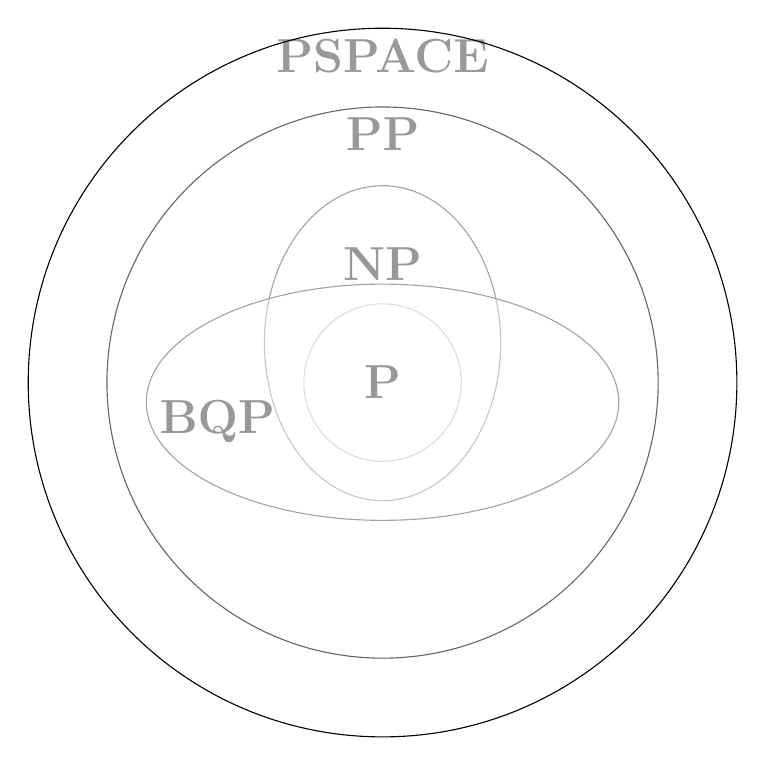
\begin{tikzpicture}
	\begin{scope} [fill opacity = .4]

    \draw[fill=white, draw = black] (0,0) circle (1);
    \draw[fill=white, draw = black] (0,0.5) ellipse (1.5 and 2);
    \draw[fill=white, draw = black] (0,-0.25) ellipse (3 and 1.5);
    \draw[fill=white, draw = black] (0,0) circle (3.5);
    \draw[fill=white, draw = black] (0,0) circle (4.5);
    
    \node at (0,0) {\LARGE\textbf{P}};
    \node at (0,1.5) {\LARGE\textbf{NP}};
    \node at (-2.1,-0.5) {\LARGE\textbf{BQP}};
    \node at (0,3.15) {\LARGE\textbf{PP}};
    \node at (0,4.15) {\LARGE\textbf{PSPACE}};
    \end{scope}

\end{tikzpicture}
\end{center}

\section{Grover's Algorithm}

Suppose we have an $F$ with only one winner $w$ (i.e., $F(w)=1$ for a unique $w$) and oracle access to $F$ through $R_F$ (see circuit above). How can we use $R_F$ to find $w$?
We might guess that we should feed (like we usually do) the equal superposition \[\ket{\psi}= \frac{1}{2^{n/2}}\sum_{x := 0}^{2^n-1}\ket{x} \] (which of course, we can prepare using $H^{\otimes n}$) into $R_F$ to get the state: \[R_F\ket{\psi}= \frac{1}{2^{n/2}}\sum_{x = 0}^{2^n-1}(-1)^{F(x)}\ket{x} = -\frac{\ket{w}}{2^{n/2}} + \frac{1}{2^{n/2}}\sum_{x \neq w}\ket{x}.\]
But what did $R_f$ do to $\ket{\psi}$?

Let us define the (unnormalized) state
\[\ket{w^{\perp}} = \frac{1}{2^{n/2}}\sum_{x \neq w}\ket{x}, \] which is orthogonal to $\ket{w}$. 

Geometrically, $R_F$ reflects $\ket{\psi}$ across the $w^{\perp}$ axis in the ``$w,w^{\perp}$'' plane, as shown in the figure below.

This does not ``help''! But at the very least, it did not hurt. (Note even though in the picture $R_F$ seems to make $\ket{\psi}$ even further from $w$, considered as quantum states (which are only distinct up to global phases), $R_F\ket{\psi}$ is exactly as close to $\ket{w}$ as $\ket{\psi}$.)

But maybe we can do something else to $R_F\ket{\psi}$ to move it closer to $\ket{w}$?\dots What if we reflect it across $\ket{\psi}$ now? Call this operation $R_{\ket{\psi}}$.

\begin{center}
    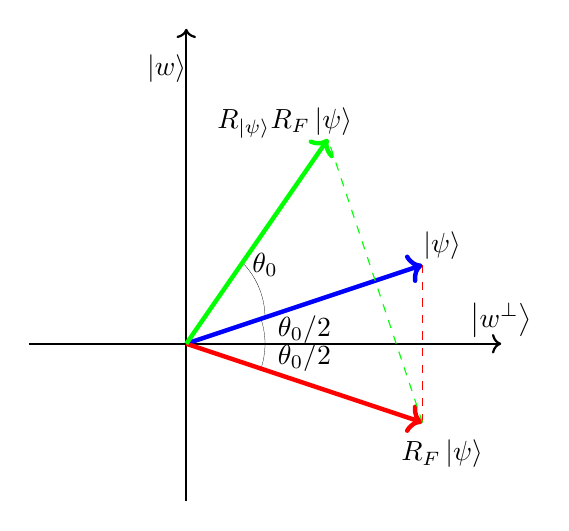
\begin{tikzpicture}
        \draw[black, thick, ->] (0,-2) -- (0,4);
        \node at (-0.25,3.5) {$\ket{w}$};
        \draw[ultra thin] (1,0) arc (0:20:1);
        \node at (1.5,0.18) {$\theta_0/2$};
        \draw[ultra thin] (1,0) arc (0:-20:1);
        \node at (1.5,-0.18) {$\theta_0/2$};
        \draw[ultra thin] (1,0.33) arc (0:45:1);
        \node at (1,1) {$\theta_0$};
        \draw[black, thick, ->] (-2,0) -- (4,0);
        \node at (4,0.3) {$\ket{w^{\perp}}$};
        \draw[blue, ultra thick, ->] (0,0) -- (3,1);
        \node at (3.25,1.25) {$\ket{\psi}$};
        \draw[red, ultra thick, ->] (0,0) -- (3,-1);
        \node at (3.25,-1.4) {$R_F\ket{\psi}$};
        \draw[green, ultra thick, ->] (0,0) -- (1.8,2.6);
	\draw[red,dashed] (3,1) -- (3,-1);
	\draw[green,dashed] (3,-1) -- (1.8,2.6);
        \node at (1.25,2.8) {$R_{\ket{\psi}}R_F\ket{\psi}$};
    \end{tikzpicture}
\end{center}


You might notice in the figure that we are assuming $\ket{\psi}$ is closer to $\ket{w^{\perp}}$ than to $\ket{w}$.  Well, this is correct as long as $n>1$, because there is only one $w$ with $f(w)=1$, but $\psi$ is the equal superposition of all $x \in \{0,1\}^n$.\footnote{The angle $\theta_0/2$ in the figure is exaggerated for clarity but it's actually very small.  Then again, it is not \emph{too} small, and this pedantic sounding point, in fact, is exactly why Grover's algoirthm works as well as it does!} In particular, if we apply $R_{\ket{\psi}}R_F$ to $\ket{\psi}$, we move \emph{closer} to $\ket{w}$ by angle $\theta_0$.  We call $R_{\ket{\psi}}R_F$ the \emph{Grover iteration} or \emph{Grover operator}.  The basic idea of Grover's algorithm is that if we apply $R_{\ket{\psi}} R_F$ the ``correct" number of times---let's call this number $r$---then we can move $\ket{\psi}$ to be very close to $\ket{w}$.\footnote{Note that we cannot just pick $r$ ``really" big like $r = 2^{n}$, since then we will rotate $\ket{\psi}$ too far!}

To make this work, we need to understand two things:
\begin{enumerate}
	\item That we can implement $R_{\ket{\psi}}$ with a quantum circuit, and
	\item What $r$ is, which will essentially amount to understanding all the angles in the figure.
\end{enumerate}		

Let's address the first point first.
Note that $R_{\ket{\psi}}$ has nothing to do with either $R_F$ or $\ket{w}$. In the $w,w^{\perp}$ plane, we can describe $R_{\ket{\psi}}$ by:
\[R_{\ket{\psi}} = 2  \ket{\psi}\bra{\psi} - \mathbb{I} \\ = 2H^{\otimes n}\ket{0}\bra{0} H^{\otimes n} - \mathbb{I} \\ = 2H^{\otimes n}\ket{0}\bra{0} H^{\otimes n} - H^{\otimes n}\mathbb{I}H^{\otimes n} = H^{\otimes n}(2\ket{0}\bra{0}-\mathbb{I})H^{\otimes n}\]
We know how to implement $H^{\otimes n}$, so it remains to show how to implement $R_g := 2\ket{0}\bra{0}-\mathbb{I}$ with a quantum circuit. As a sanity check, note that $R_g$ is in fact a unitary on all of $\qbits{n}$; in fact, $R_g$ is exactly the ``phase oracle" for the Boolean function $g$ where

	\[\begin{aligned}
	g: \{0,1\}^n &\to \{0,1\}\\
	0 &\mapsto 0 \\
    0\neq x &\mapsto 1
	\end{aligned}\]
In other words, $g(x_1, \dotsb, x_n)=OR(x_1, \dotsb, x_n) = OR(x_1, OR(x_2, \dotsb, x_n))$ is a big OR of all its inputs.  Obviously we can implement this using a classical Boolean circuit with $n-1$ many standard 2-ary OR gates.  Thus:
    $R_g$ can be implemented with a quantum circuit of size poly($n$).

Now let's address the second point, which is arguably more interesting.
From the figure, $\theta_0$ is twice the angle between $\ket{\psi}$ and $\ket{w^{\perp}}$. We can use the inner product to figure out this angle. In general, \[\cos \angle(u,v) = \frac{|\braket{u}{v}|}{\norm{u}\norm{v}}.\] For our case, \[\theta_0 = 2\arccos (\frac{|\braket{\psi}{w^{\perp}}|}{\norm{\psi}\norm{w^{\perp}}}).\] We have $\norm{\psi}=1$, \[\norm{w^{\perp}} = \sqrt{\braket{w^{\perp}}{w^{\perp}}} = \sqrt{\frac{2^n-1}{2^n}} = \sqrt{1-\frac{1}{2^n}}\], and $|\braket{\psi}{w^{\perp}}|= \frac{2^n-1}{2^n}$. So,
\[\theta_0 = 2\arccos(\sqrt{1-\frac{1}{2^n}}),\] from which we get (using trigonometry) \[\sin^2(\theta_0/2)=\frac{1}{2^n}.\] Now using the Taylor expansion for arcsin \[\theta_0= 2\arcsin(\sqrt{\frac{1}{2^n}})= 2 \sqrt{\frac{1}{2^n}}+\mathcal{O}(2^{-3n/2})=\Theta(\frac{1}{2^{n/2}})\]

On the other hand, the angle between $\ket{\psi}$ and $\ket{w}$ is essentially $90^{\circ}$ (but not exactly, otherwise the Grover iteration would not make any progress)! Angle $\angle(\ket{\psi},\ket{w})$ satisfies \[\angle(\ket{\psi},\ket{w}) = \frac{\pi}{2}-\frac{\theta_0}{2}=\frac{\pi}{2} - \Theta(2^{-n/2})\]

Each application of $R_{\ket{\psi}}R_F$ rotates the plane by $\theta_0$. So, if we do this operation exactly $r \sim 2^{n/2}$ times, the angle between $(R_{\ket{\psi}}R_F)^r\ket{\psi}$ and $\ket{w}$ will be within $2^{-n/2}$ of $0$.

Therefore, if we measure $(R_{\ket{\psi}} R_F)^r \ket{\psi}$ in the computational basis, then with probability greater than $2/3$ (there are some minor fudge factors here), we will get outcome $w$.  Since each application of $R_{\ket{\psi}} R_F$ requires exactly one call of $R_F$ and $r \sim 2^{-n/2}$, this is exactly what we wanted to show!

\end{document}